\section{Antecedentes}
	
	Para esta investigación se buscaron antecedentes de alcance nacional e internacional que ayuden a guiar, sustentar y validar esta investigación.
	
	\textcite{casallas2005desarrollo}, escribieron para la revista Acción Pedagógica de la Universidad de los Andes un artículo titulado \enquote{Desarrollo básico de un Laboratorio Virtual de Control de Procesos basado en Internet}, fue desarrollado conjuntamente entre la UNET y la ULA para ser usado a través de Internet y cuyo objetivo fue desarrollar un laboratorio virtual de control de procesos para la enseñanza a distancia, permitiendo ser utilizado solo por usuarios registrados y en determinados horarios. Aunque la finalidad de la investigación acá propuesta difiere del objetivo de \citeauthor{casallas2005desarrollo}, esta servirá como ayuda para determinar las funciones más utilizadas en el área de control, así como las necesidades típicas de un laboratorio de control virtual.
	
	Adicionalmente, \textcite{salazar2019diseno}, realizo en la Universidad Técnica del Norte, Ecuador, una tesis titulada \enquote{Diseño de un sistema de riego inteligente para cultivos de hortalizas basado en Fuzzy Logic en la granja la pradera de la Universidad Técnica del Norte.} para la implementación del controlador basado en la lógica difusa utilizo, entre otros equipos, un Rasberry PI para la ejecución de Python, específicamente, hizo uso de la biblioteca Scikit-Fuzzy, la cual le permitió definir las funciones de membresía, establecer las reglas difusas, realizar los procesos de fuzzificación y defuzzificación, todo esto para una arquitectura de controlador difuso tipo Mamdani, esta tesis servirá como referencia para establecer el diseño de controladores difusos utilizando la biblioteca Scikit-Fuzzy.

	Por otro lado, \textcite{congo2018aplicaciones} realizo en la Universidad Tecnológica Israel, Ecuador, una tesis titulada \enquote{Aplicaciones del software libre Python para prácticas de laboratorio aplicado a la asignatura de tratamiento digital de señales de la Universidad Tecnológica Israel} cuyo objetivo fue desarrollar por medio del software Python y sus diferentes librerías científicas, la realización de 3 Prácticas de Laboratorio para la asignatura Procesamiento Digital de Señales de la Universidad Tecnológica Israel, al igual que la intención de este trabajo, se realizó una interfaz gráfica con el objetivo de facilitar su uso, en este caso como herramienta para el procesamiento digital de señales. Este trabajo sustenta la viabilidad de realizar una interfaz gráfica con enfoque similar en el campo de la electrónica y se utilizara como guía parcial para establecer su uso en sistemas de control.
	
	Finalmente, \textcite{cadavid2009toolbox} redacto para la revista Educación en Ingeniería de Colombia, un artículo titulado \enquote{Toolbox didáctico para el diseño y análisis de sistemas de control lineal}, cuyo objetivo es describir un toolbox realizado en MATLAB para el análisis de sistemas de control lineales, este toolbox consiste de una interfaz gráfica que permite realizar pruebas a sistemas de control como respuesta escalón, respuesta en frecuencia, análisis de estabilidad, diseño de controladores, entre otras funciones. Este articulo será de utilidad para establecer la interfaz gráfica que se pretende realizar, además, sirvió como punto de partida para determinar las funciones que debería tener un laboratorio virtual de sistemas de control, como punto adicional se puede resaltar que reafirma la utilidad de esta investigación. 
	
\section{Bases teóricas}
	
    Para poder realizar el laboratorio virtual de sistemas de control clásicos y difusos será necesario abarcar conocimientos de análisis de sistemas de control, diseño de controladores PID y controladores difusos, a continuación, se presentan los conceptos necesarios para el desarrollo de esta investigación.
    
    \subsection{Procesos}
		
		Es importante partir de la base, es por ellos que empezaremos con los procesos, \textcite{sanchez2003control} define los procesos como \enquote{[...] un bloque que se identifica porque tiene una o más variables de salida de las cuales es importante conocer y mantener sus valores}(p.$\,$153). Así, un proceso se caracteriza por tener una entrada y una salida (para procesos SISO), dicha salida deberá mantenerse alrededor de un punto de referencia dado, es decir, se debe controlar su salida.
	
	\subsection{Modelado de procesos en tiempo continuo}
	
		Un proceso puede ser representado por ecuaciones diferenciales que determinen su comportamiento dinámico en el dominio del tiempo, no obstante, trabajar con ecuaciones diferenciales es tedioso a nivel matemático, por tanto, se prefiere modelar los procesos utilizando la transformada de Laplace para llevar de una representación dinámica a una algebraica, esta ecuación algebraica se operara para llevar a una función de transferencia que represente al proceso en el dominio de la frecuencia compleja \Parencite{smith1985principles}.
	
		\subsubsection{Transformada de Laplace}
		
			La transformada de Laplace de una función dependiente del tiempo f(t) viene dada por la ecuación:
			
			\begin{equation}\label{eq:Laplace}
				F(s) = \mathcal{L}\left[f(t) \right] = \int_{0}^{\infty} f(t)e^{-st}dt
			\end{equation}
			
			\noindent si suponemos que f(t) es un proceso cuya representación dinámica viene dada por una ecuación diferencial de la forma:
			
			\begin{equation}\label{eq:Diffeq}
				a_{2}\frac{d^{2}y(t)}{dt^{2}} + a_{1}\frac{dy(t)}{dt} + a_{0}y(t) = b_{0}x(t)
			\end{equation}
			
			Aplicando \cref{eq:Laplace} a \cref{eq:Diffeq}  y despejando la relación $Y(s)/X(s)$ para el proceso con condiciones iniciales igual a cero (debido a que el proceso debe ser lineal) se obtiene la correspondiente función de transferencia del proceso $H(S)$:
			
			 \begin{equation}\label{eq:TransferFunction}
			 	H(s) =	\frac{Y(s)}{X(s)} = \frac{b_{0}}{a_{2}s^{2} + a_{1}s + a_{0}}
			 \end{equation}
			 
			 La demostración completa \Parencite[pp.$\,$21-22]{smith1985principles} no es de interés para este trabajo, pero si su resultado, la función de transferencia puede ser analizada para determinar las características del proceso, como su ganancia, constante de tiempo, tiempo muerto, entre otras.
			 
		 \subsubsection{Ecuaciones de espacio de estado}
		 
		 	Las ecuaciones de espacio de estado son un método más moderno para modelar todo tipo de sistemas, no solo físicos, sino también biológicos, económicos, sociales y otros. Así como una ecuación diferencial puede ser representada como una función de transferencia también se puede representar como una ecuación de espacio de estados, por tanto, una función de transferencia también puede ser representada en el espacio de estados y viceversa. Las ecuaciones linealizadas alrededor de un estado de operación \Parencite[p.$\,$31]{ogata2003ingenieria} son:
		 
			\begin{align}
                \dot{x}(t) &= Ax(t) + Bu(t) \label{eq:SSrepresentationX} \\
				y(t) &= Cx(t) + Du(t) \label{eq:SSrepresentationY}
			\end{align}
			
			\begin{spacing}{1.5}
				\noindent con: 
				
				$A$: como matriz de estado.
				
				$B$: como matriz de entrada.
				
				$C$: como matriz de salida.
				
				$D$: como matriz de transmisión directa.
				
            \end{spacing}
            
            Normalmente la notación presentada en las ecuaciones \cref{eq:SSrepresentationX,eq:SSrepresentationY} es preferida dado que son compactas y fáciles de entender, no obstante, es al expandir las ecuaciones en su forma matricial que podemos ver claramente que la ecuación \cref{eq:SSrepresentationX} es un sistema de ecuaciones diferenciales ordinarias:
            
            \vspace{20pt}
            \begin{align}
                \begin{bmatrix}
                    \dot{x}_{1}\\
                    \dot{x}_{2}\\
                    \vdots\\
                    \dot{x}_{n}\\
                    \end{bmatrix}&=
                    \begin{bmatrix}
                    a_{11} & a_{12} & \cdots & a_{1n}\\
                    a_{21} & a_{22} & \cdots & a_{2n}\\
                    \vdots & \vdots & \ddots & \vdots\\
                    a_{n1} & a_{n2} & \cdots & a_{nn}\\
                    \end{bmatrix}
                    \begin{bmatrix}
                    x_{1}\\
                    x_{2}\\
                    \vdots\\
                    x_{n}\\
                    \end{bmatrix}+
                    \begin{bmatrix}
                    b_{11} & b_{12} & \cdots & b_{1m}\\
                    b_{21} & b_{22} & \cdots & b_{2m}\\
                    \vdots & \vdots & \ddots & \vdots\\
                    b_{n1} & b_{n2} & \cdots & b_{nm}\\
                    \end{bmatrix}.
                    \begin{bmatrix}
                    u_{1}\\
                    u_{2}\\
                    \vdots\\
                    u_{m}\\
                    \end{bmatrix}\label{eq:FullSSx}\\
                    \begin{bmatrix}
                    y_{1}\\
                    y_{2}\\
                    \vdots\\
                    y_{n}\\
                    \end{bmatrix}&=
                    \begin{bmatrix}
                    c_{11} & c_{12} & \cdots & c_{1n}\\
                    c_{21} & c_{22} & \cdots & c_{2n}\\
                    \vdots & \vdots & \ddots & \vdots\\
                    c_{r1} & c_{r2} & \cdots & c_{rn}\\
                    \end{bmatrix}
                    \begin{bmatrix}
                    x_{1}\\
                    x_{2}\\
                    \vdots\\
                    x_{n}\\
                    \end{bmatrix}+
                    \begin{bmatrix}
                    d_{11} & d_{12} & \cdots & d_{1m}\\
                    d_{21} & d_{22} & \cdots & d_{2m}\\
                    \vdots & \vdots & \ddots & \vdots\\
                    d_{r1} & d_{r2} & \cdots & d_{rm}\\
                    \end{bmatrix}.
                    \begin{bmatrix}
                    u_{1}\\
                    u_{2}\\
                    \vdots\\
                    u_{m}\\
                    \end{bmatrix}
            \end{align}
            \vspace{20pt}

            \begin{spacing}{1.5}
				\noindent con: 
				
				$n$: como el numero de variables de estado
				
				$m$: como el numero de entradas
				
				$r$: como el numero de salidas
				
            \end{spacing}

            Para resolver estos sistemas de ecuaciones diferenciales podemos utilizar metodos iterativos como los metodos de Runge-Kuuta.

    \subsection{Modelado de procesos en tiempo discreto}

        Así como para tiempo continuo se utilizan ecuaciones diferenciales, en el tiempo discreto se hace uso de ecuaciones en diferencias, las ecuaciones en diferencias se pueden utilizar para aproximar a las ecuaciones diferenciales, estas primeras se suelen utilizar porque son más fáciles de programar \Parencite{kuo1996sistemas}, debido a esto los procesos pueden ser representados de la siguiente forma:
        
        \begin{equation}\label{eq:EqEnDiferencias}
            y(k+n) + a_{n-1}y(k+n-1) + \cdots + a_1 y(k+1) + a_0 y(k) = f(k) 
        \end{equation}
        
        Asi mismo debido a que la ecuacion \cref{eq:SSrepresentationX} esta compuesta de ecuaciones diferenciales, esta puede ser llevada a una ecuacion en diferencias y la representacion del proceso en el espacio de estados queda como sigue:

        \begin{align}\label{eq:SSdiscreto}
            x(k+1) &= A_d x(k) + B_d u(k) \\
            y(k) &= C_d x(k) + D_d u(k)
        \end{align}

        \subsubsection{Transformada z}
		
			En tiempo discreto se puede modelar un proceso utilizando la transformada z sobre la ecuación en diferencias del proceso para obtener su representacion en el dominio Z, la transformada Z es a las ecuaciones en diferencia lo que la transformada de laplace es las ecuaciones en tiempo continuo, la ecuación general para la transformada z es:
			
			\begin{equation}\label{eq:Ztransform}
				F(z)= \sum\limits_{k=0}^{\infty}f(k)z^{-k}
			\end{equation}

        \subsubsection{Discretizacion de una funcion de transferencia continua}
            
            Existen varios metodos para realizar la discretizacion de una funcion de transferencia continua, el metodo mas simple suele implicar el uso de un muestreador con un retensor de orden zero (ZOH), retensor de orden zero significa que la señal de entrada es retenida constantemente durante el intervalo de muestreo \Parencite{haugen2005discrete}, la formula para realizar la discretizacion con retensor de orden zero es la siguiente:

            \begin{equation}\label{eq:ZOH}
                H(z) = (1 - z^{-1}) \mathcal{Z} \left[ \mathcal{L}^{-1}\left\lbrace \frac{G(s)}{s}\right\rbrace\Bigr|_{t=kh}\right]
            \end{equation}

            Existen otros modos de llevar una función de transferencia continua al dominio Z como las aproximaciones de Tustin y Euler, estas consisten en sustituir la variable s por una aproximación en el dominio Z y se sustentan en ser aproximaciones numéricas a integrales en el tiempo, \textcite{haugen2005discrete} afirma que la aproximacion de Tustin es la mas precisa de las tres, no obstante, sugiere que no existe una diferencia notable entre este y Euler hacia atrás, ademas, la mayoría de los controladores comerciales vienen con Euler hacia atrás, por lo que puede considerarse una mejor opción a la hora de escoger un método. Las sustituciones correspondientes son:

            \begin{align}
                &\text{Euler hacia adelante:}& &s \leftarrow \frac{z - 1}{h} \label{eq:eulerF}\\
                &\text{Euler hacia atrás:}& &s \leftarrow \frac{z - 1}{hz} \label{eq:eulerB}\\
                &\text{Tustin:}& &s \leftarrow \frac{2}{h} \frac{z-1}{z+1} \label{eq:tustin}
            \end{align}
    
    \subsection{Respuesta en el tiempo del modelo en el espacio de estados}
        
        Para poder obtener la respuesta del sistema en el tiempo podemos utilizar varios metodos de resolucion de ODE's o ecuaciones diferenciales ordinarias, solucion exacta, separacion de variables o integracion numerica aproximada, este ultimo es el mejor para realizar por medio de computadoras. Para realizar la integracion numerica y obtener la respuesta del sistema se utilizaran los metodos de Runge-Kutta.

        Los metodos de Runge-Kutta son unos metodos iterativos de resolucion de ODE's, estos se basan en utilizar \blockquote[{\cite[p.31]{horacio1997metodos}}]{indirectamente el algoritmo de Taylor. En general, estos metodos evaluan $f(x,y)$ en mas de un punto en la proximida $(x_n,y_n)$ en lugar de evaluar derivdas de $f(x,y)$}. La formulacion general de los metodos de Runge-Kutta explicitos es:
        
        \begin{equation}\label{eq:RKgeneral}
            \begin{aligned}
                k_1 &= f(x_0,y_0)\\
                k_2 &= f(x_0 + c_2 h,y_0 + ha_{21}k_1)\\
                k_3 &= f(x_0 + c_3 h,y_0 + h(a_{31}k_1 + a_{32}k_2))\\
                &\mathrel{\makebox[\widthof{=}]{\vdots}}\\
                k_s &= f(x_0 + c_s h,y_0 + h(a_{s1}k1 + \cdots +  a_{s,s-1}k_{s-1}))\\
                y_1 &= y_0 + h(b_1 k_1 + \cdots + b_s k_s)
            \end{aligned}
        \end{equation}
        
        Donde $s$ denota el numero de escenarios a utilizar, es comun expresar \cref{eq:RKgeneral} utilizando una tabla de butcher, en honor a John C. Butcher y su articulo de 1964b, por tanto, \cref{eq:RKgeneral} puede representarse de la siguiente forma:

        \begin{equation}\label{eq:explicitoButcher}
            \renewcommand\arraystretch{1.2}
            \begin{array}
            {c|ccccc}
            0\\
            c_2 & a_{21}\\
            c_3 & a_{31} & a_{32}\\
            \vdots & \vdots & \vdots & \ddots\\
            c_s & a_{s1} & a_{s2} & \cdots & a_{s,s-1}\\
            \hline
            & b_1 & b_2 & \cdots & b_{s-1} &  b_{s}
            \end{array}
        \end{equation}

        Adicionalmente existen los metodos de Runge-Kutta embebidos, los cuales consisten en calcular dos metodos de orden $p$ y orden $\hat{p}$ respectivamente, donde $\hat{p}$ es normalmente $p-1$ o $p+1$ \Parencite{hairer1991solving}. La tabla de butcher para representar los metodos embebidos es la siguiente:

        \begin{equation}\label{eq:embebidoButcher}
            \renewcommand\arraystretch{1.2}
            \begin{array}
            {c|ccccc}
            0\\
            c_2 & a_{21}\\
            c_3 & a_{31} & a_{32}\\
            \vdots & \vdots & \vdots & \ddots\\
            c_s & a_{s1} & a_{s2} & \cdots & a_{s,s-1}\\
            \hline
            & b_1 & b_2 & \cdots & b_{s-1} &  b_{s}\\
            \hline
            & \hat{b}_1 & \hat{b}_2 & \cdots & \hat{b}_{s-1} &  \hat{b}_{s}
            \end{array}
        \end{equation}

        \begin{align}
            y_1 &= y_0 + h(b_1 k_1 + \cdots + b_s k_s) & &\text{Orden $p$}\\
            \hat{y}_1 &= y_0 + h(\hat{b}_1 k_1 + \cdots +\hat{b}_s k_s) & &\text{Orden $\hat{p} = p-1$ o $p+1$}
        \end{align}

        De modo que la integración para el siguiente paso se continua con $y_1$, el fin de calcular dos metodos en conjunto es para poder estimar el error y poder realizar un cambio en el tamaño de paso, de este modo, se puede incrementar el tamaño de paso si el error es muy bajo o disminuirlo si el error es inaceptable.
        
        \subsubsection{Runge-Kutta's para ecuaciones de espacio de estados}

            Partiendo de la ecuacion \cref{eq:FullSSx} en donde podemos observar que $\dot{x}(t)$ viene dado por un conjunto de ecuaciones diferenciales ordinarias, por tanto, es posible aplicar los metodos de Runge-Kutta de forma casi directa, \textcite{horacio1997metodos} desarrolla las expresiones para un Runge-Kutta de orden 4 aplicado en el espacio de estados, estas expresiones pueden ser extendidas para generalizar su aplicacion a un numero de escenarios arbitrarios, el vector de estados de forma general se puede expresar como:

            
            \begin{equation}\label{eq:vectorGeneral}
                \begin{aligned}
                    x_1(t) &= f_1(t, x_1, x_2, \dots, x_n) = f_1(t,x)\\
                    &\mathrel{\makebox[\widthof{=}]{\vdots}}\\
                    x_n(t) &=  f_n(t,x)
                \end{aligned}
            \end{equation}

            \noindent cuyas condiciones iniciales se pueden expresar como:

            \begin{equation}\label{eq:vectorIniciales}
                \begin{aligned}
                    x_1^{(0)} &= \alpha_1\\
                    &\mathrel{\makebox[\widthof{=}]{\vdots}}\\
                    x_n^{(0)} &=  \alpha_n
                \end{aligned}
            \end{equation}
            
            \noindent de modo que al sustituir \cref{eq:vectorGeneral,eq:vectorIniciales} en \cref{eq:RKgeneral} y señalando:

            \vfill 

            \begin{spacing}{1.5}
				
				$n$: como el numero de variables de estado
				
				$m$: como el numero de entradas
				
				$j$: como la iteracion actual
                
                $s$: como el numero de escenarios
            \end{spacing}

            \vfill
            \pagebreak

            \noindent se obtenga el nuevo vector de estado:

            \begin{equation}\label{eq:RKstate}
                \begin{aligned}
                    k_1 &= Ax_n^{(j)} + Bu_m^{(j)}\\
                    k_2 &= A(x_n^{(j)} +  ha_{21}k_1) + Bu_m^{(j)}\\
                    k_3 &= A(x_n^{(j)} +  h(a_{31}k_1 + a_{32}k_2)) + Bu_m^{(j)}\\
                    &\mathrel{\makebox[\widthof{=}]{\vdots}}\\
                    k_s &= A(x_n^{(j)} + h(a_{s1}k1 + \cdots +  a_{s,s-1}k_{s-1})) + Bu_m^{(j)}\\
                    x_n^{(j+1)} &= x_n^{(j)} + h(b_1 k_1 + \cdots + b_s k_s)
                \end{aligned}
            \end{equation}
            
            \noindent finalmente, el vector de estado obtenido con \cref{eq:RKstate} sera sustituido en la siguiente iteraciones, para obtener la salida actual se debe sustituir $x_n^{(j)}$  en \cref{eq:SSrepresentationY}. 
            
            \begin{equation}
				y^{(j)} = Cx_n^{(j)} + Du_m^{(j)} \label{eq:SSrepresentationY}
            \end{equation}
            
            Estos pasos se repiten una y otra vez de forma iterativa utilizando un tamaño de paso adecuado, el tamaño de paso determinara el numero de iteraciones a realizar, un tamaño de paso pequeño genera resultados mas precisos pero incrementa el tiempo de computo considerablemente, por otro lado, un tamaño de paso grande puede generar errores inaceptables con la ventaja de acelerar los cálculos, el tamaño de paso es un factor muy importante en los metodos de Runge-Kutta.

        \subsubsection{Tamaño de paso variable}

            Como ya se menciono antes, se puede realizar una adaptacion del tamaño de paso en funcion del error, esto es posible no solo para los metodos embebidos, sino también para los explícitos, \textcite{roganprogramacion} afirma que: \blockquote[p.251]{Los programas adaptativos continuamente monitorean la solución y modifican el paso de
            tiempo para asegurar que se mantenga la precisión especificada por el usuario. Esos programas
            pueden hacer algunos cálculos extras para optimizar la elección de $\tau$ , en muchos casos este
            trabajo extra vale la pena.}
            
            \paragraph{Calculo del error con dos medios pasos}

                Este es un metodo simple pero eficaz de calcular el error, consiste en realizar un paso simple de tamaño h y comparar su respuesta con la respuesta dada por el mismo método al realizar dos pasos de tamaño $\frac{h}{2}$, de este modo el error $\Delta e$ se puede calcular como la diferencia en valor absoluto de ambas respuestas, $\left|y_{1,h} - y_{2,\frac{h}{2}}\right|$ donde $y_{2,\frac{h}{2}}$ es la salida luego de dos medios pasos.
            
            \paragraph{Calculo del error para metodos embebidos} 

                Los metodos embebidos están hechos para poder realizar este calculo del error, por tanto, no hay que realizar ningún calculo extra y el error puede ser calculado de forma directa como $\Delta e = \left| y_1 - \hat{y}_1\right|$

            \paragraph{Nuevo tamaño de paso}

                Combinando las formulas y algoritmos descritos por \textcite{roganprogramacion}, \textcite{hairer1991solving} y \textcite{ritschel2013numerical} se pueden obtener las formulas para el manejo del error con fines de calcular un nuevo tamaño de paso, lo primero es calcular una escala, este es el único paso que se diferencia entre el método de dos medios pasos y el los metodos embebidos, esto es debido a al modo en que se calculan los errores, para dos medios pasos la escala es:

                \begin{equation}\label{eq:escalaDos}
                    escala = atol + rtol \cdot \frac{\left|y_{1,h}\right| + \left|y_{2,\frac{h}{2}}\right|}{2}
                \end{equation}

                \noindent para los metodos embebidos:

                \begin{equation}\label{eq:escalaEmbebidos}
                    escala = atol + rtol \cdot max(\left| y_1\right|,\left| y_0\right|)
                \end{equation}
        
                A partir de aca las formulas son comunes para ambos metodos. Para continuar, se debe realizar el calculo de un error normalizado, para esto se calcula la norma RMS del error dividido por la escala calculada:

                \begin{equation}\label{eq:ErrorNormalizado}
                    ||\Delta e|| = \sqrt{\frac{1}{n} \sum_{i=1}^{n} \left(\frac{\Delta e_i}{escala_i}\right)^2}
                \end{equation}

                \noindent donde i denota el numero de elementos que componen la respuesta, finalmente, el nuevo tamaño de paso viene dado por:
                
                \begin{equation}
                    \left\{
                    \begin{aligned}
                        h_{t+1} &= h_{t}\cdot maxStepIncrease &\quad &Si \quad ||\Delta e|| = 0\\
                        h_{t+1} &= h_{t}\cdot sf_1 \cdot ||\Delta e||^{\frac{-1}{q+1}}  &\quad &Si \quad ||\Delta e|| \leq 1 \\
                        h_{t} &= h_{t}\cdot sf_1 \cdot ||\Delta e||^{\frac{-1}{q+1}}  &\quad &Si \quad ||\Delta e|| > 1 \ ,\ \text{Se descarta la salida}
                    \end{aligned}\right.
                \end{equation}
                
                \noindent con $sf_1$ como un factor de seguridad que evita que el nuevo tamaño de paso para un $||\Delta e||$ dado se repita indefinidamente, y $q$ como el orden del metodo utilizado, en el caso de los Runge-Kutta embebidos, $q$ viene dado por el metodo de menor orden entre $y_1$ y $\hat{y}_1$, notese que si el error se encuentra por arriba de uno, la salida es descartada y se repite el calculo con un nuevo tamaño de paso, el proceso se repite hasta que el error sea igual o menor que uno.
    
    \subsection{Respuesta en el tiempo del modelo en el espacio de estados discreto}
        
        El calculo de la respuesta en el tiempo para el modelo en el espacio de estados discreto es mucho mas simple, no se requiere ningun metodo de integracion aproximado, esto es debido a que el calculo puede ser realiado se forma directa, esto es debido a que la formula es el algoritmo a seguir \Parencite{haugen2005discrete}. Tomando en consideracion la ecuacion \cref{eq:SSdiscreto}, basta con sustituir el vector de estado para obtener a $x(k+1)$ y la salida $y(k)$
    
    \subsection{Sistemas de control}
		
		\subsubsection{Sistema en lazo abierto}
		
            Un sistema en lazo abierto es aquel cuya salida no es medida en ningún momento en orden de ajustar la entrada, esto provoca que \enquote{las perturbaciones que se presentan en el proceso ocasionen que sus efectos se sientan en la salida del proceso, es decir, en el valor de la variable controlada}\Parencite[p.$\,$350]{maloney2006electronica}. La mayoría de los sistemas en lazo abierto son estables, pero carecen de utilidad practica al no poder mantenerlos en un punto de referencia debido a las perturbaciones.
            
            Por otro lado, es importante analisar el comportamiento del sistema en lazo abierto para determinar su comportamiento en lazo cerrado, ademas, nos permite determinar sus caracteristicas con el fin de realizar un modelo matematico aproximado del sistema, este es util para realizar la entonacion de los controladores sin tener que trabajar de forma directa con el proceso, el cual puede ser peligroso o inaccesible. La representacion en diagrama de bloques de un sistema en lazo abierto se puede observar en la \cref{fig:esquemaLazoAbierto}.
            
            \begin{figure}[htb]
				\centering
				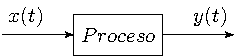
\includegraphics[width=0.5\textwidth]{esquemaLazoAbierto.pdf}
				\caption[Ejemplo de un sistema en lazo abierto]{\textbf{Sistema en lazo abierto}. Fuente: Elaboración propia.} 
				\label{fig:esquemaLazoAbierto}
            \end{figure}
        
        \subsubsection{Sistema en lazo cerrado}
		
			Los sistemas de lazo cerrado son aquellos cuya salida es realimentada a la entrada del sistema, esta realimentación suele ser negativa para que sea estable, no obstante, existen sistemas que se vuelven inestables con el simple hecho de cerrar el lazo, un ejemplo de sistema realimentado se puede observar en la \cref{fig:esquemaLazoCerrado}.
			
			\begin{figure}[htb]
				\centering
				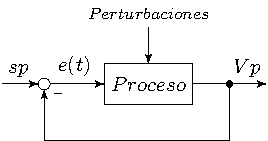
\includegraphics[width=0.6\textwidth]{esquemaLazoCerrado.pdf}
				\caption[Ejemplo de un sistema en lazo cerrado]{\textbf{Sistema en lazo cerrado}. Se observan las principales señales de un sistema en lazo cerrado. Fuente: Elaboración propia.} 
				\label{fig:esquemaLazoCerrado}
			\end{figure}
			
            En la \cref{fig:esquemaLazoCerrado} se denotan algunas de las señales que componen a un sistema de control, $sp$, que corresponde al set point o valor de referencia, $Vp$, que corresponde a la variable del proceso y es la variable a controlar, las perturbaciones, las cuales son magnitudes físicas que pueden afectar al proceso como la temperatura ambiente, presión, vibraciones, entre otras, y finalmente, $e(t)$, que corresponde a la señal de error la cual viene dada por la diferencia entre el valor de referencia y la variable medida \Parencite{maloney2006electronica}.
            
            \begin{equation}\label{eq:Serror}
				e(t) = sp - Vp
            \end{equation}
            
        \subsubsection{Estabilidad de los sistemas}

            La estabilidad se ve afectada por la estructura del sistema, por tanto, se debe tomar en cuanta cuando se cierra el lazo del sistema. \textcite{ogata2003ingenieria} afirma que, desde el punto de vista de estabilidad, el sistema de control en lazo abierto no es un problema importante. Por otra parte, la estabilidad es un gran problema en el sistema de control en lazo cerrado debido a la posibilidad de que se generen oscilaciones. Esto quiere decir que los análisis de estabilidad se realizan para sistemas en lazo cerrado, esto es principalmente porque los sistemas en lazo abierto tienden a ser estables, además, para realizar el control de un proceso se suele utilizar los sistemas en lazo cerrado

            \paragraph{Análisis de estabilidad en el plano complejo}
            
                La estabilidad de un sistema lineal viene dada por la ubicación de sus polos a lo largo del plano complejo s, tomando esto en cuenta se puede determinar si un sistema es estable si no posee ninguno polo en el semiplano derecho del plano complejo s incluyendo el eje coordenado $j\omega$ en tiempo continuo \Parencite{ogata2003ingenieria}, en el caso de sistemas discretos, los polos deben encontrarse dentro del circulo unitario, la estabilidad marginal es posible si existen uno o mas polos justo en el circulo unitario, pero no multiples. Esto permite que el análisis de estabilidad se pueda realizar de forma analítica y gráfica. En la \cref{fig:pzmap} se puede observar dos sistemas continuos en lazo abierto, $G_1(s)$ que es estable y $G_2(s)$ que es inestable .

                \begin{figure}[htb]
                    \centering
                    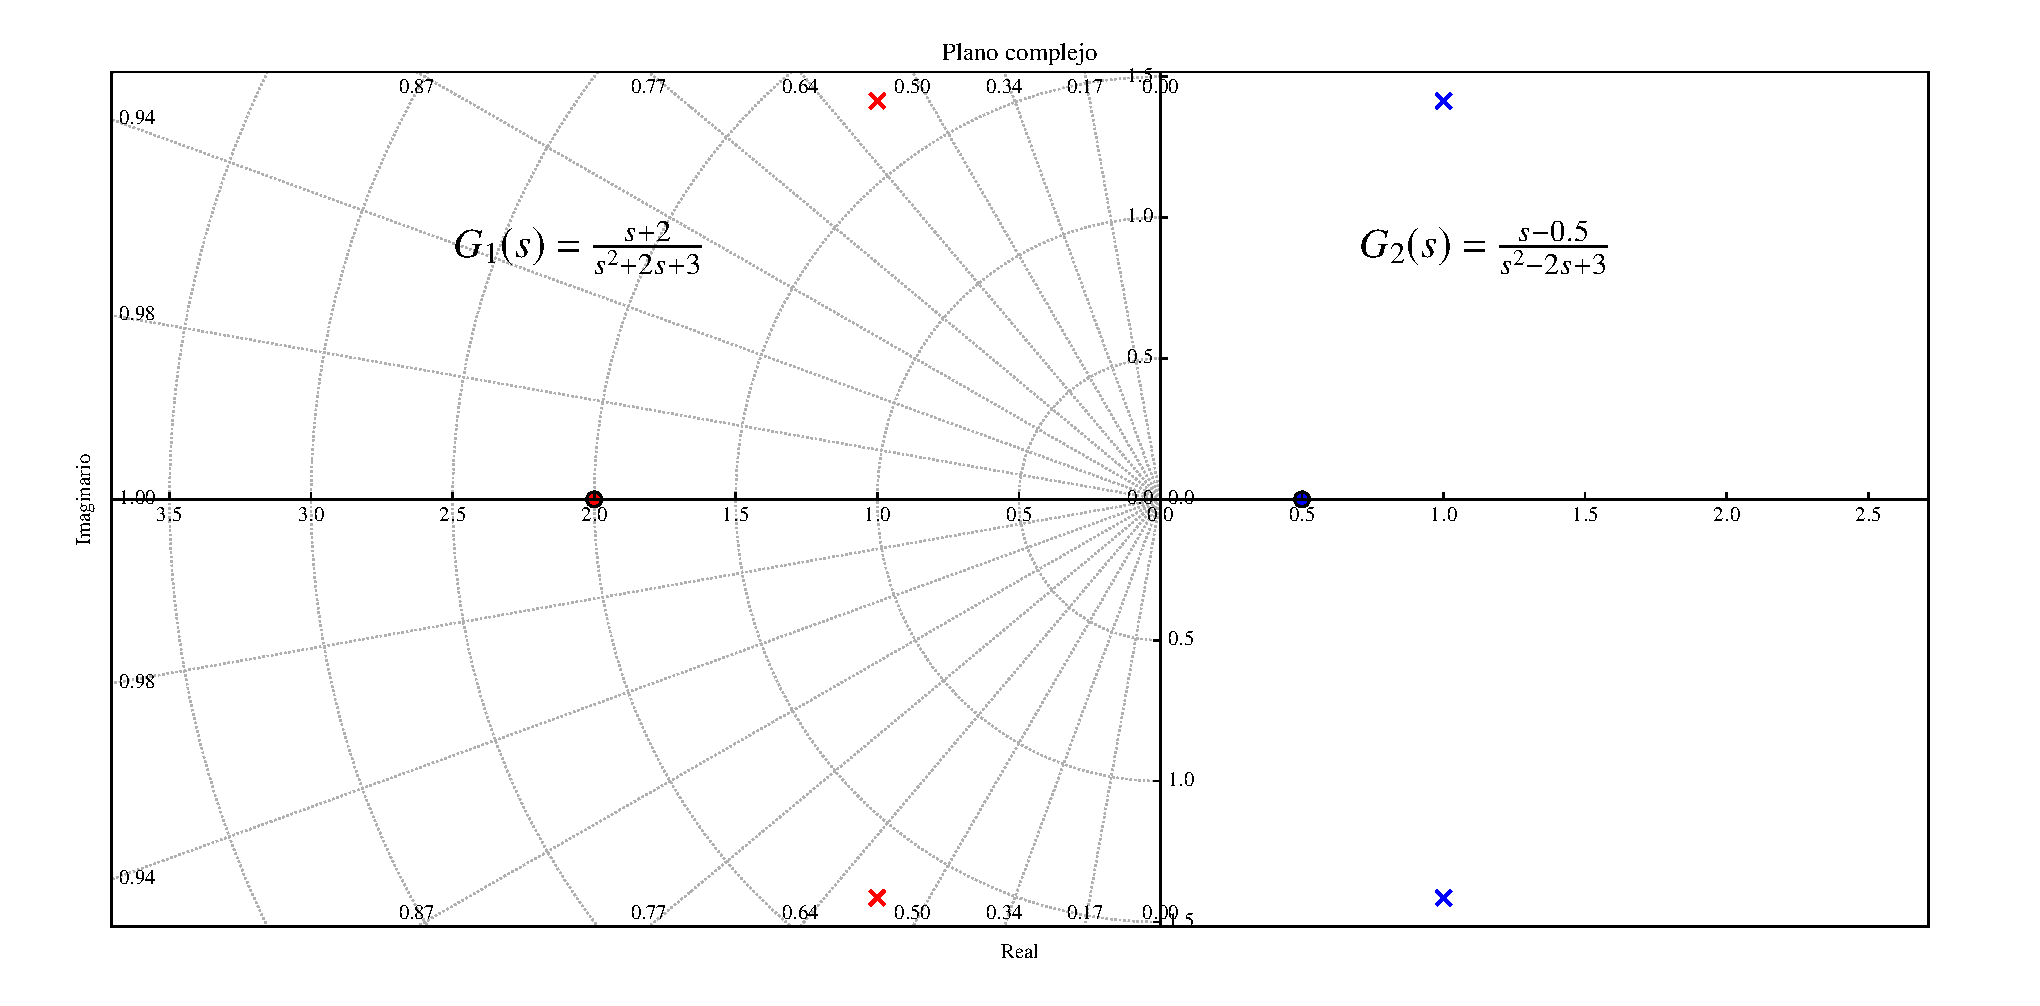
\includegraphics[width=\textwidth]{pzmap.pdf}
                    \caption[Ejemplo de analisis de estabilidad en el plano complejo]{\textbf{Analisis de estabilidad en el plano complejo}. Se puede observar como el sistema $G_1(s)$ tiene ubicado sus polos en el semiplano izquierdo del plano complejo, i.e., es estable, por otro lado, el sistema $G_2(s)$ es inestable al poseer polos ubicados en el semiplano derecho del plano complejo. Fuente: Elaboración propia.} 
                    \label{fig:pzmap}
                \end{figure}
            
            \paragraph{Criterio de estabilidad de Nyquist}
                
                El criterio de estabilidad de Nyquist determina el estado de estabilidad utilizando los polos en lazo abierto y la respuesta en frecuencia del sistema en lazo abierto, este criterio \enquote{es útil en la ingeniería de control, debido a que permite determinar gráficamente la estabilidad absoluta del sistema en lazo cerrado a partir de las curvas de respuesta en frecuencia en lazo abierto, sin que sea necesario determinar los polos en lazo cerrado}\Parencite[p.$\,$446]{ogata2003ingenieria}. Este criterio tiene la ventaja de poder realizarse tanto con cálculos analíticos como con datos experimentales, \textcite{ogata2003ingenieria} define tres criterios:

                \begin{enumerate}[leftmargin=\parindent]
                    \item El punto $-1 + j0$ no esta rodeado. Esto implica que el sistema es estable en lazo cerrado si no hay polos de $G(s)H(s)$ en el semiplano derecho del plano s\footref{fn:continuevsdiscreto}; de lo contrario, el sistema es inestable.
                    \item El punto $-1 + j0$ queda rodeado una o varias veces en sentido contrario al de las agujas
                    del reloj. En este caso, el sistema es estable en lazo cerrado si el número de rodeos en sentido contrario
                    al de las agujas del reloj es igual al número de polos $G(s)H(s)$ en el semiplano derecho
                    del plano s\footref{fn:continuevsdiscreto}; de lo contrario, el sistema es inestable.

                    \footnotetext[1]{En el caso de sistemas discretos se toma en cuenta son los polos fuera del circulo unitario para la evaluacion de los criterios. \label{fn:continuevsdiscreto}}

                    \item El punto $-1 + j0$ queda rodeado una o varias veces en el sentido de las agujas del reloj.
                    En este caso el sistema es inestable en lazo cerrado.
                \end{enumerate}
                
                En la \cref{fig:nyquistPlot} se puede observar los diagramas de Nyquist para los sistemas presentados en la \cref{fig:pzmap}, el sistema $G_1(s)$ debe ser evaluado por el criterio numero 1, al no poseer ninguno polo en el semiplano derecho el sistema sera estable en lazo cerrado asumiendo un $H(s) = 1$, por otro lado, $G_2(s)$ debe ser evaluado por el criterio numero 2, debido a que el numero de rodeos al punto $-1 + j0$ es igual al numero de polos en el semiplano derecho, el sistema sera estable en lazo cerrado asumiendo un $H(s) = 1$, esto a pesar de que en lazo abierto sea inestable.

                \begin{figure}[htb]
                    \centering
                    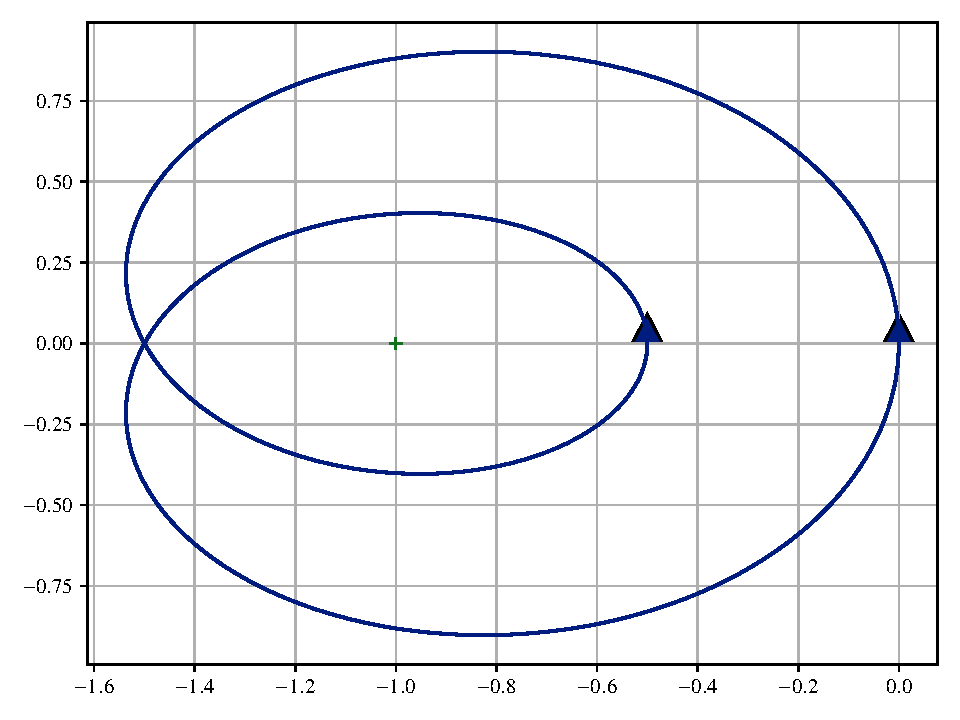
\includegraphics[width=0.7\textwidth]{nyquistPlot.pdf}
                    \caption[Ejemplo de analisis de estabilidad con diagrama de Nyquist]{\textbf{Analisis de estabilidad con diagrama de Nyquist}. El sistema $G_1(s)$ al ser evaluado con el criterio numero 1 se encuentra que es estable en lazo cerrado, a su vez, el sistema $G_2(s)$ al ser evaluado con el criterio numero 2 se encuentra que tambien sera estable en lazo cerrado, en ambos casos se asume un $H(s) = 1$. Fuente: Elaboración propia.} 
                    \label{fig:nyquistPlot}
                \end{figure}
            
            \paragraph{Margen de ganancia y Margen de fase}
                
                Los margenes de ganancia y de fase son una medida de la estabilidad relativa, se toma en cuenta a la hora de realizar el diseño de un controlador, esto es debido a que los margenes se pueden interpretar de modo que orienten en la cantidad de ganancia que se le puede aplicar al sistema en lazo cerrado, adicionalmente, la estabilidad relativa se puede interpretar como que tan estable es un sistema.
                    
            \paragraph{Análisis de estabilidad con las trazas de Bode}

                Los diagramas de bode son una forma de representar la respuesta en frecuencia de un sistema tomando en cuenta los cambios de amplitud de $H(j\omega)$ y del ángulo de fase de $H(j\omega)$ respecto a la frecuencia \Parencite{nilsson1995circuitos}. Para analizar la estabilidad se utilizan el margen de ganancia y el margen de fase del sistema en un diagrama de Bode a modo de trazas, creando así, zonas claramente delimitadas por estas trazas que determinan la estabilidad relativa del sistema dependiendo de la zona en donde se ubiquen en función de $\omega$.

                 


                

                